\documentclass{beamer}

\usepackage[utf8]{inputenc}
\usetheme{Antibes}

\usepackage{fontspec}
\setmainfont{Times New Roman}
\setsansfont{Arial}
\newfontfamily\greekfont[Script=Greek]{Linux Libertine O}
\newfontfamily\greekfontsf[Script=Greek]{Linux Libertine O}
\usepackage{polyglossia}
\setdefaultlanguage{greek}

\usepackage{color, colortbl}
%\usepackage[table,xcdraw]{xcolor}
\usepackage{minted}
\usepackage{amsmath}
\usepackage{amssymb,longtable}
\usepackage{bm}
\usepackage{changepage}
\usepackage{tikz}
\usepackage{tikz-qtree}
\usepackage{url}
\usepackage{booktabs,makecell}
\usepackage{diagbox}

\usetikzlibrary{calc}
\usetikzlibrary{arrows.meta}
\usetikzlibrary{positioning}
%% I define a "style" for the "cells"
\tikzset{
  my cell/.style={
    draw,
    minimum size=5ex,
    node distance=0pt,
  }}
%% to make changing appearances for various aspects of
%% the diagram easier, I define several macros which need
%% only be changed here.  Even though two of these macros
%% have the same definition, I use two to allow the possibility
%% that these styles could be diffferent.
\newcommand\mynodestyle{\sffamily}
\newcommand\myrelocatestyle{\sffamily\bfseries}
\newcommand\mynumberstyle{\sffamily}

\DeclareMathSymbol{\mlq}{\mathord}{operators}{``}
\DeclareMathSymbol{\mrq}{\mathord}{operators}{`'}
\newcommand*\circled[1]{\tikz[baseline=(char.base)]{
   \node[shape=circle,draw,inner sep=1pt] (char) {#1};}}

\tikzset{%
	>={Latex[width=2mm,length=2mm]},
  	% Specifications for style of nodes:
	base/.style = {rectangle, rounded corners, draw=black,
				   minimum width=4cm, minimum height=1cm,
				   text centered, font=\sffamily},
	factory/.style = {base, fill=blue!30},
	parser/.style = {base, fill=red!30},
	ast/.style = {base, fill=green!30},
	process/.style = {base, minimum width=2.5cm, fill=orange!15,
					  font=\ttfamily},
}

%Information to be included in the title page:
\title[Μελέτη και βελτίωση της επίδοσης του συντακτικού αναλυτή Packrat] % optional
{Μελέτη και βελτίωση της επίδοσης του συντακτικού αναλυτή Packrat}

\author[Νίκος, Μαυρογεώργης] % (optional, for multiple authors)
{Νίκος Μαυρογεώργης}

\institute[ECE, NTUA] % (optional)
{
  Σχολή Ηλεκτρολόγων Μηχανικών και Μηχανικών Υπολογιστών\\
  Εθνικό Μετσόβειο Πολυτεχνείο
}

\date[NTUA 2020] % (optional)
{Παρουσίαση Διπλωματικής \\ Ιούλιος 2020 \\ Επιβλέπων Καθηγητής: Νίκος Παπασπύρου}

\AtBeginSection[]
{
  \begin{frame}
    \frametitle{Πίνακας Περιεχομένων}
    \tableofcontents[currentsection]
  \end{frame}
}

\begin{document}

\frame{\titlepage}

\begin{frame}
\frametitle{Πίνακας Περιεχομένων}
\tableofcontents
\end{frame}

\section{Εισαγωγή}

\begin{frame}
  \frametitle{Συντακτική Ανάλυση}
  \begin{itemize}	
	\item Πρακτικά όλες οι γλώσσες, είτε φυσικές είτε γλώσσες μηχανής, βασίζονται στην έκφραση της πληροφορίας με γραμμικό τρόπο
	\item Συνήθως η αναπαράσταση γίνεται με τη μορφή μίας \textit{συμβολοσειράς}, που είναι μια ακολουθία χαρακτήρων από ένα τυποποιημένο σύνολο
	\item Οποιαδήποτε εφαρμογή επεξεργασίας γλώσσας πρέπει να μετατρέψει τις συμβολοσειρές σε πιο αφηρημένες δομές όπως λέξεις, φράσεις, προτάσεις, εκφράσεις ή εντολές \pause
  \end{itemize}

\begin{block}{Ορισμός}
  \textit{Συντακτική ανάλυση (parsing)} είναι η διαδικασία που εξάγει χρήσιμη δομημένη πληροφορία από γραμμικό κείμενο.
\end{block}

\end{frame}

\begin{frame}
  \frametitle{Πόσο κοστίζει η συντακτική ανάλυση?} \pause
  \begin{itemize}
	\item Αποτελεί σημαντικό κομμάτι της εκτέλεσης προγραμμάτων, ειδικά στις διερμηνευόμενες γλώσσες όπου οι εντολές δεν μετατρέπονται σε ένα εκτελέσιμο, αλλά εκτελούνται διαρκώς εκ νέου:
  \begin{itemize}
	\item Γλώσσες Σεναρίων: Python, Javascript
	\item Γλώσσες Σήμανσης: HTML, CSS, Postscript
	\item Γλώσσες ανταλλαγής δεδομένων: XML, JSON \pause
  \end{itemize}
\item Κατά το rendering ιστοσελίδων, η συντακτική ανάλυση των HTML, CSS και Javascript καταναλώνει έως και το 40\% της διαδικασίας. \pause
  \end{itemize}

  \begin{block}{Συμπέρασμα}
	Θα άξιζε να μειώναμε το χρόνο εκτέλεσής της, ιδιαίτερα αν αξιοποιούσαμε και τα πολυπύρηνα συστήματα που είναι σχεδόν πάντα διαθέσιμα.
  \end{block}
\end{frame}

\begin{frame}
  Σε ποιες γραμματικές απευθύνεται το packrat?
\end{frame}

\section{Parsing Expression Grammars}

\begin{frame}
  \frametitle{Parsing Expression Grammars - Κίνητρο}

  \begin{itemize}
	\item Οι δύο πιο συνηθισμένες μέθοδοι για να περιγραφεί η σύνταξη μίας γλώσσας: οι κανονικές εκφράσεις και οι γραμματικές χωρίς συμφραζόμενα (CFGs) \pause
	\item Ένα ακόμη χρήσιμο πρότυπο περιγραφής της σύνταξης είναι οι \textit{Parsing Expression Grammars (PEGs)} 
	\item Μοιάζουν με τις γραμματικές χωρίς συμφραζόμενα, αλλά έχουν και ορισμένες θεμελιώδεις διαφορές  \pause
	\item Δαισθητικά μια CFG μας περιγράφει το πώς  \textit{κατασκευάζεται} μία συμβολοσειρά που ανήκει σε κάποια γλώσσα, ενώ οι  PEGs  το πώς  \textit{αναλύεται} η συμβολοσειρά ώστε να προκύψει δομική πληροφορία για αυτή
  \end{itemize}

\end{frame}
\begin{frame}
  \frametitle{Parsing Expression Grammars - Κίνητρο}
  \begin{example}
Γλώσσα από τη συνένωση ζευγών $\mathbf{a}$
	\begin{itemize}
	  \item Παραγωγικός ορισμός: $\{ s \in \mathbf{a}^* | s = {(\mathbf{a}\mathbf{a})}^n\}$ δηλαδή μια γλώσσα με ένα μόνο γράμμα στο λεξιλόγιό της της οποίας οι συμβολοσειρές 
 κατασκευάζονται συνενώνοντας ζεύγη από $ \mathbf{a}$
      \item Αναγνωριστικός ορισμός: $\{ s \in \mathbf{a}^* | (\lvert s \rvert mod2=0)\}$ δηλαδή μία συμβολοσειρά από $\mathbf{a}$'s γίνεται αποδεκτή μόνο αν το μήκος της είναι άρτιο
	\end{itemize}
  \end{example}
\pause
Ο σχεδιαστής της γραμματικής είναι ευκολότερο να σκέφτεται πώς αναλύεται μία δοσμένη συμβολοσειρά στα συστατικά της, παρά πώς θα γεννηθεί (generated) η συμβολοσειρά μέσα από τους κανόνες της γραμματικής.
\end{frame}

\begin{frame}
  \frametitle{Parsing Expression Grammars - Ορισμοί}
  \begin{itemize}
	\item Κανόνες της μορφής `$ n \leftarrow e $', όπου $ n$ μη τερματικό και $e$ έκφραση ("για να αναγνωρίσεις το $n$, αναγνώρισε πρώτα το $e$") \pause
	  \item Αριστερό βέλος αντί για δεξί: διασθητική διαφορά στην "ροή της πληροφορίας" \pause
	  \item Oι κανόνες των CFGs εκφράζουν "παραγωγές" από μη τερματικά στις αντίστοιχες εκφράσεις τους ενώ των  PEGs αναπαριστούν "αφαιρέσεις" από τις εκφράσεις στους αντίστοιχους κανόνες
  \end{itemize}
  \end{frame}

\begin{frame}
  \frametitle{Parsing Expression Grammars - Εκφράσεις}

 \begin{description}[font=$\bullet$\scshape\bfseries]
   \item[Κενή συμβολοσειρά `()' :] "Μην προσπαθήσεις να διαβάσεις τίποτα: απλά επίστρεψε επιτυχώς χωρίς να καταναλώσεις τίποτα από την είσοδο." \pause

   \item[Τερματικό `$ \alpha$':] "Αν το επόμενο τερματικό στην είσοδο είναι $ \alpha $ τότε κατανάλωσε ένα τερματικό και επίστρεψε επιτυχώς. Αλλιώς, απότυχε και μην καταναλώσεις τίποτα."\pause

   \item[Μη Τερματικό `$ A $':] "Προσπάθησε να διαβάσεις την είσοδο με βάση τον κανόνα που αντιστοιχεί στο  $ A $ και επίστρεψε επιτυχώς ή απότυχε αντίστοιχα."
  \end{description}
\end{frame}

\begin{frame}
  \frametitle{Parsing Expression Grammars - Εκφράσεις}

 \begin{description}[font=$\bullet$\scshape\bfseries]
   \item[Ακολουθία `$(e_1 e_2 \ldots e_n)$':] "Προσπάθησε να διαβάσεις μία συμβολοσειρά ώστε να επιτύχει η $e_1$. 
	 Αν η $ e_1$ επιτύχει, κάνε το ίδιο με την  $e_2$, ξεκινώντας από το σημείο της εισόδου που δεν κατανάλωσε η  $e_1$ κ.ό.κ. 
	 Αν και οι  $n$ εκφράσεις αναγνωριστούν επίστρεψε επιτυχώς και κατανάλωσε τα αντίστοιχα κομμάτια της εισόδου.
	 Αν οποιαδήποτε υποέκφραση αποτύχει, απότυχε χωρίς να καταναλώσεις τίποτα."

  \end{description}
\end{frame}

\begin{frame}
  \frametitle{Parsing Expression Grammars - Εκφράσεις}
 \begin{description}[font=$\bullet$\scshape\bfseries]
   \item[Διατεταγμένη Επιλογή `$(e_1 / e_2 / \ldots / e_n)$':] "Προσπάθησε να διαβάσεις μία συμβολοσειρά ώστε να επιτύχει η $e_1$. 
	 Αν επιτύχει τότε η επιλογή επιστρέφει επιτυχώς καταναλώνοντας το αντίστοιχο κομμάτι της εισόδου.
	 Αλλιώς, προσπάθησε με την $e_2$ και την αρχική είσοδο κ.ό.κ, μέχρις ότου να επιτύχει κάποια από τις υποεκφράσεις.	 Αν καμία από τις $n$ εναλλακτικές δεν πετύχουν, τότε απότυχε χωρίς να καταναλώσεις τίποτα." \pause
  \end{description}
  \begin{example}
    Έστω ο κανόνας $Number \leftarrow Digit~Number / Digit$. 
	Η σειρά έχει σημασία, διότι αν ήταν ανάποδα και  θέλαμε να αναλύσουμε τον αριθμό $12$, θα πηγαίναμε πρώτα στην εναλλακτική $Digit$, θα αναγνωρίζαμε το 1 και θα επιστρέφαμε χωρίς να πάμε στο $2$.
  \end{example}

\end{frame}

\section{Packrat Parsing}

\begin{frame}
  \frametitle{Ορισμοί}
  \begin{itemize}
	\item Ο απλούστερος και διαισθητικά προφανής τρόπος να σχεδιάσουμε έναν συντακτικό αναλυτή είναι η από πάνω προς τα κάτω ανάλυση ή ανάλυση αναδρομικής κατάβασης. 
	\item \textit{Προβλέποντες (predictive) συντακτικοί αναλυτές}: επιχειρούν να προβλέψουν ποιο στοιχείο της γλώσσας ακολουθεί, βλέποντας ορισμένα από τα προπορευόμενα σύμβολα στην είσοδο.
	\item \textit{Συντακτικοί αναλυτές με οπισθαναχώρηση (backtracking)}: παίρνουν αποφάσεις υποθετικά (speculatively) και δοκιμάζουν διαδοχικά διάφορες εναλλακτικές. Aν μία αποτύχει, τότε ο αναλυτής οπισθαναχωρεί στη θέση της εισόδου που ήταν προτού δοκιμάσει την εναλλακτική και μετά εξετάζει την επόμενη εναλλακτική. \pause
  \end{itemize}

  Ποιο από τα δύο θα επιλέξουμε? \pause Και τα δύο!

  \end{frame}

\begin{frame}
  \frametitle{Θεμέλια}
  \begin{itemize}
	\item Αξιοποιούμε τη λογική της αναδρομικής κατάβασης (απλότητα), αποθηκεύοντας τα ενδιάμεσα αποτελέσματα σε έναν πίνακα, ώστε να μη χρειάζεται backtracking \pause
  \end{itemize}
  \begin{block}{Πίνακας Packrat}
	Θεωρούμε έναν πίνακα όπου το κελί $(i, j)$ περιέχει το αποτέλεσμα της συντακτικής ανάλυσης του μη τερματικού $i$, ξεκινώντας από τη θέση $j$.
\end{block}
\end{frame}

\begin{frame}
  \frametitle{Παράδειγμα}
\begin{figure}
	\begin{equation}
		\begin{array}{l}
		  \textcolor<3, 8, 10->{red}{Additive} \; \leftarrow \; Multitive \; \mlq \textcolor<10->{red}{+} \mrq \; Additive \; | \; Multitive \\
			\textcolor<9, 7>{red}{Multitive} \; \leftarrow \; Primary \; \mlq * \mrq \; Multitive \; | \; Primary \\
			\textcolor<6>{red}{Primary} \; \leftarrow \; \mlq ( \mrq \; Additive \; \mlq ) \mrq \; | \; Decimal \\
			\textcolor<5>{red}{Decimal} \; \leftarrow \; \mlq 0 \mrq \; | \; ... \; | \; \mlq 9 \mrq \; 
		\end{array}
	\end{equation}
\end{figure}
\pause
\begin{longtable}{lllllllll}
    column & C1 & C2& C3& C4& C5& C6& C7& C8 \\
    \hline
	Additive&  & & $\uparrow$& \textcolor<3, 11->{red}{(7,C7)}& \textcolor<9->{orange}{X}& \textcolor<8->{orange}{(4,C7)}& \textcolor<4->{orange}{X}& \textcolor<4->{orange}{X} \\
	Multitive& &  & \vdots & \textcolor<9->{orange}{(3,C5)}& \textcolor<9->{orange}{X}& \textcolor<7->{orange}{(4,C7)}& \textcolor<4->{orange}{X}& \textcolor<4->{orange}{X} \\
	Primary &   & $\leftarrow$ \ldots & \circled{?}& \textcolor<9->{orange}{(3,C5)}& \textcolor<9->{orange}{X}& \textcolor<6->{orange}{(4,C7)}& \textcolor<4->{orange}{X}& \textcolor<4->{orange}{X} \\
	Decimal &  & & Χ& \textcolor<9->{orange}{(3,C5)}& \textcolor<9->{orange}{X}& \textcolor<5->{orange}{(4,C7)}& \textcolor<4->{orange}{X}& \textcolor<4->{orange}{X}\\
    \hline
	Input String & '2'& '*' & '('& '3'& '\textcolor<10->{red}{+}'& '4'& ')'& EOF\\
	\\
\end{longtable}

\end{frame}

\begin{frame}
  \frametitle{Υπομνηματισμός}
  \begin{itemize}
	\item Δεν χρειάζεται να υπολογίσουμε όλα τα ενδιάμεσα κελιά
	\item Ξεκινάμε με αναδρομή από το αρχικό σύμβολο στην αρχή της εισόδου και αποθηκεύουμε τα ενδιάμεσα αποτελέσματα που υπολογίζουμε (memoisation) \pause
	\item Ακόμα και backtracking να γίνει κανένα κελί δεν θα χρειαστεί να ξαναυπολογιστεί \pause $\rightarrow$ γραμμικός αλγόριθμος! \pause
  \end{itemize}

\begin{figure}[h]
    \centering
	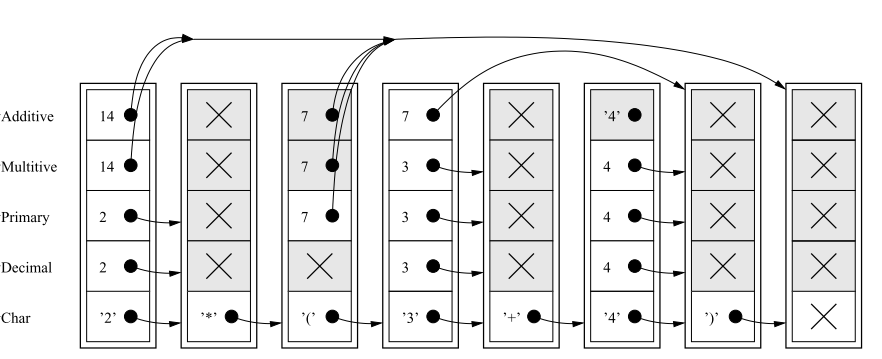
\includegraphics[width=0.85\textwidth]{../transcript/pics/packrat_memo_example}
\end{figure}

\end{frame}

\begin{frame}
  \frametitle{Υλοποίηση - PEG}
\begin{figure}[h]
    \centering
	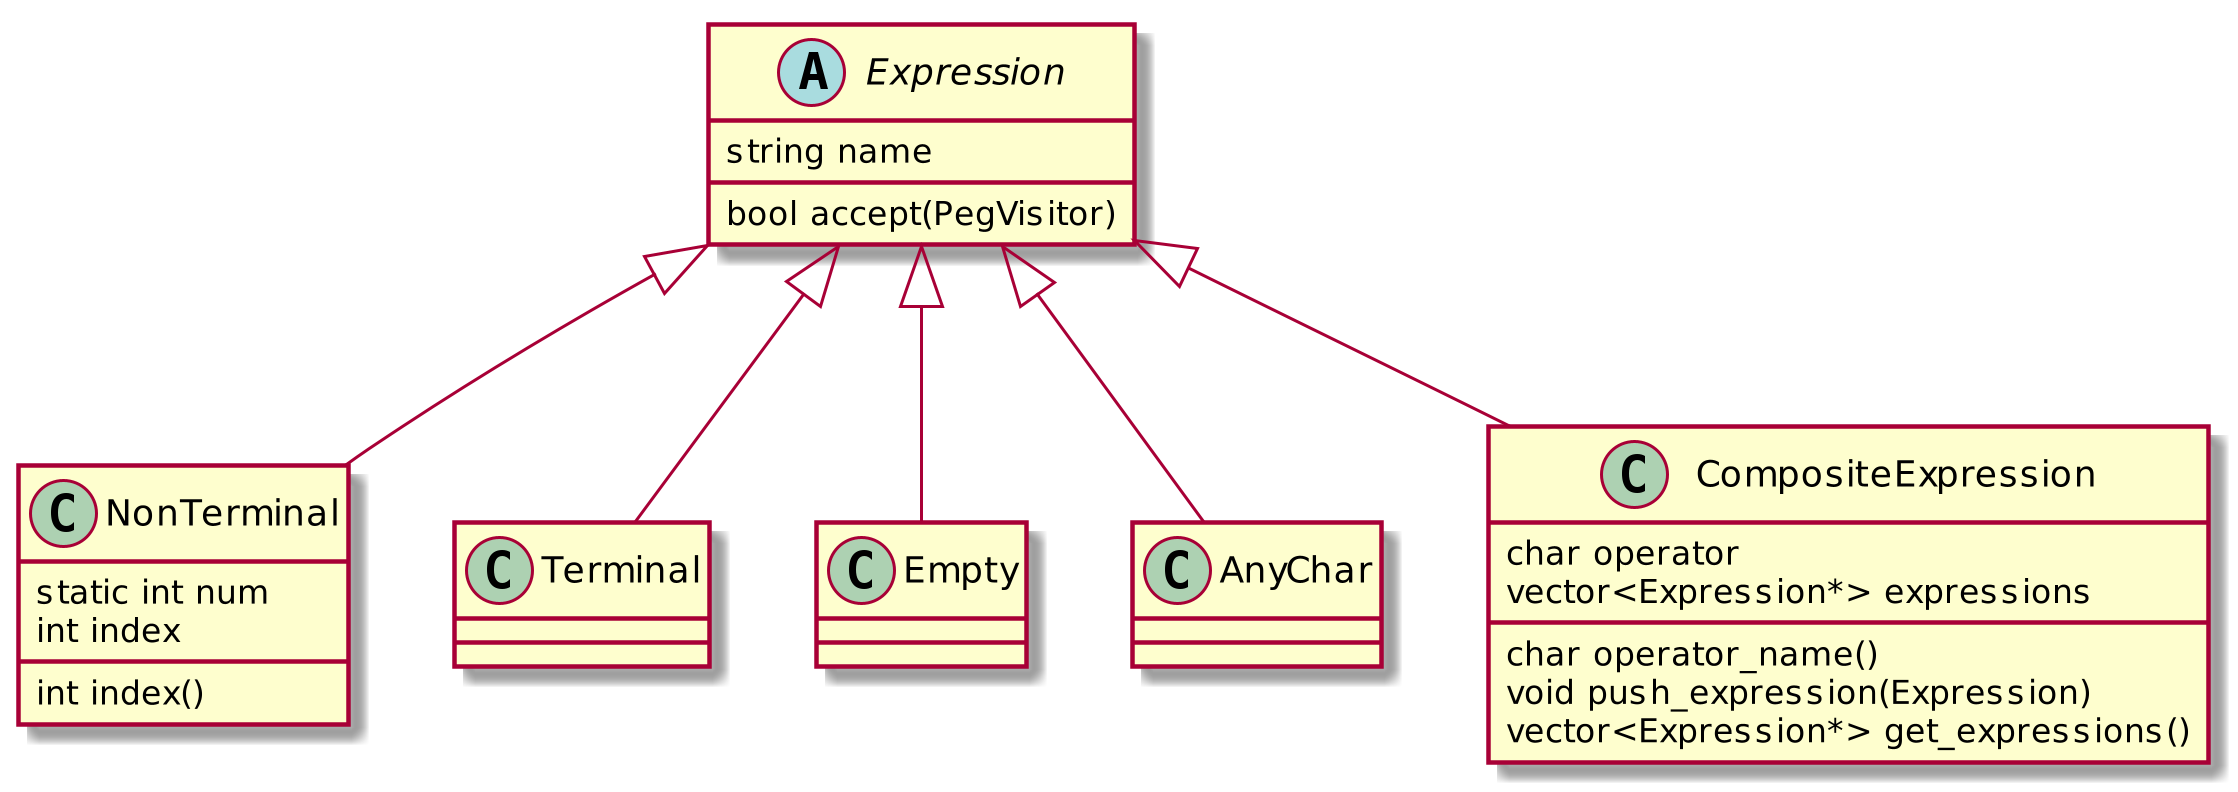
\includegraphics[width=1.05\textwidth]{../transcript/uml/peg_elements}
\end{figure} \pause
\begin{figure}[h]
    \centering
	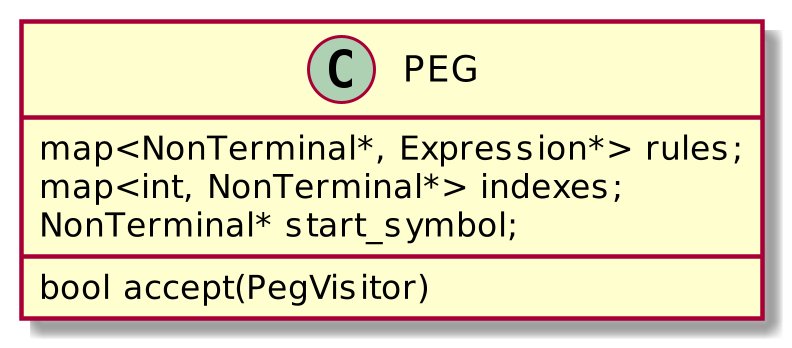
\includegraphics[width=0.40\textwidth]{../transcript/uml/peg}
\end{figure}
\end{frame}

\begin{frame}
  \frametitle{Υλοποίηση - Packrat}
\begin{figure}[h]
    \centering
	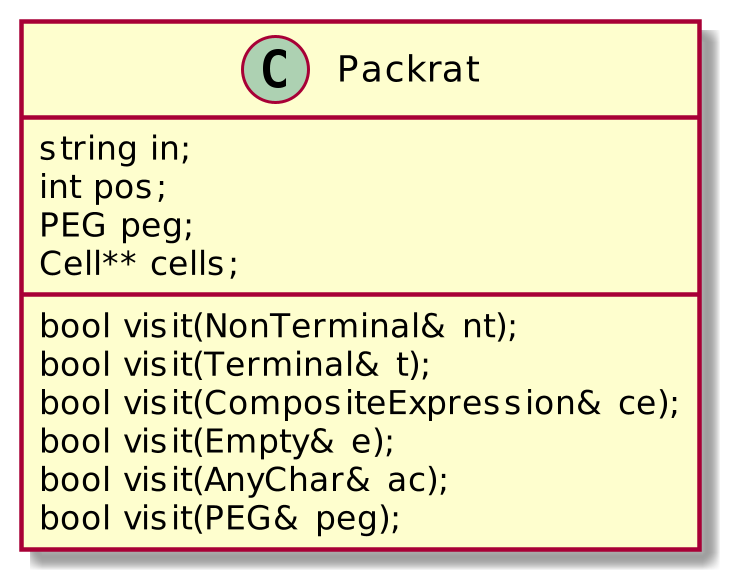
\includegraphics[width=0.60\textwidth]{../transcript/uml/packrat}
\end{figure} 
\end{frame}

\begin{frame}[fragile]
  \frametitle{Υλοποίηση - Visit Terminal}
\begin{figure}[h]
    \centering
	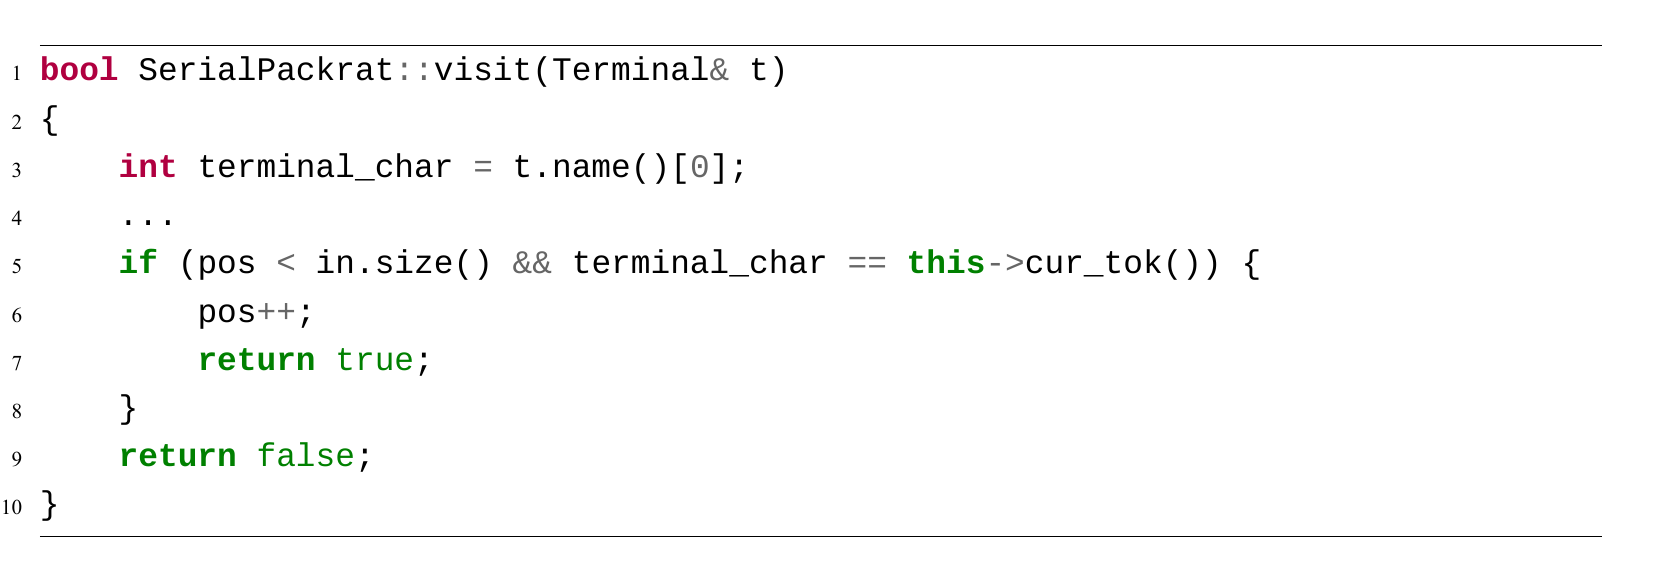
\includegraphics[width=1.10\textwidth]{pics/terminal}
\end{figure} 
\end{frame}

\begin{frame}
  \frametitle{Υλοποίηση - Visit Non Terminal}

\begin{columns}

\column{0.5\textwidth}
\begin{figure}[h]
    \centering
	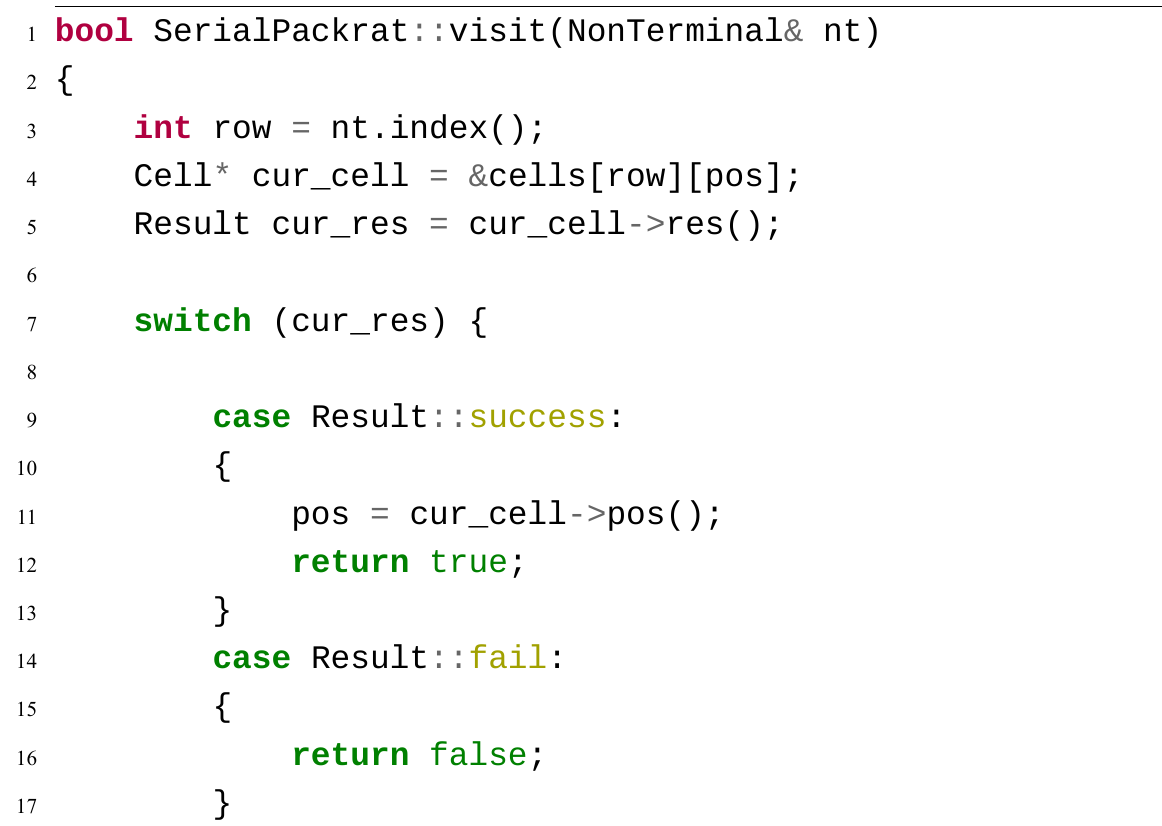
\includegraphics[width=1.10\textwidth]{pics/nt_1}
\end{figure} 

\column{0.5\textwidth}
\begin{figure}[h]
    \centering
	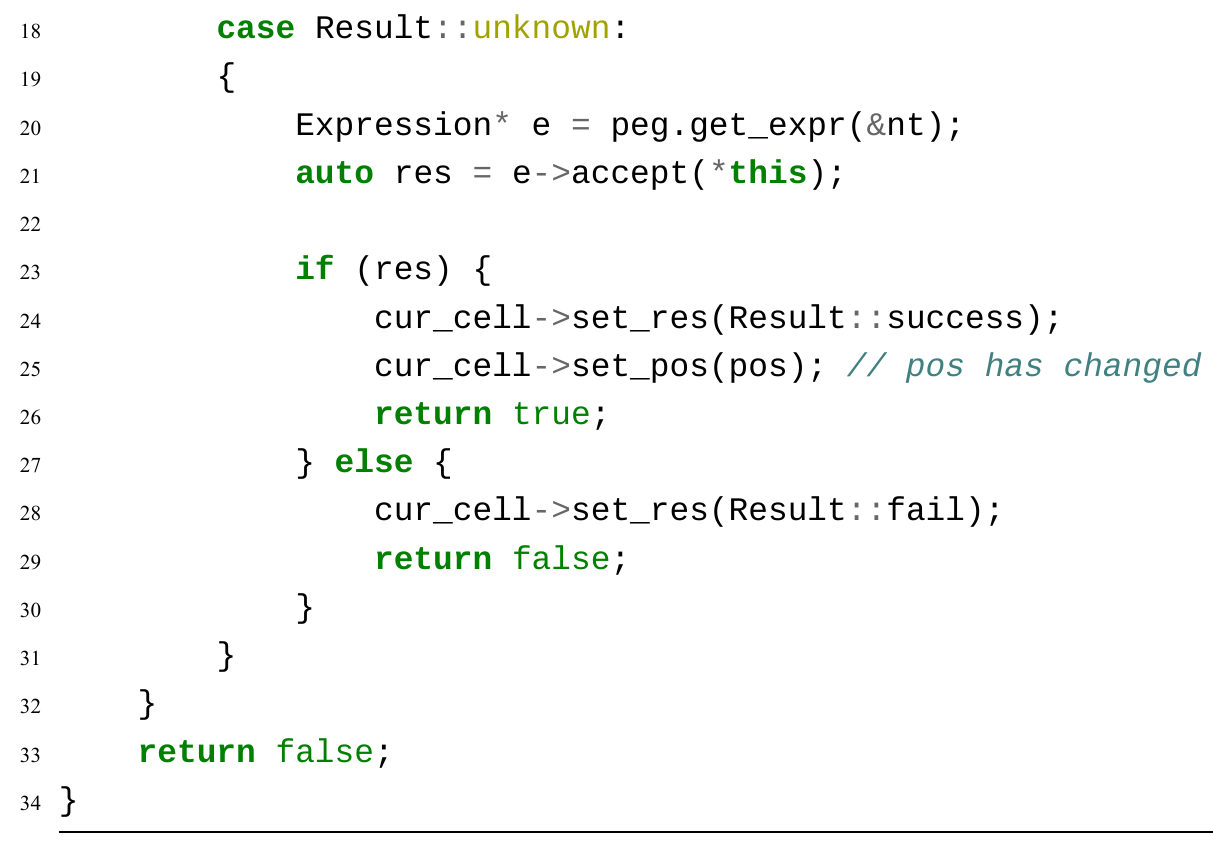
\includegraphics[width=1.10\textwidth]{pics/nt_2}
\end{figure} 

\end{columns}

\end{frame}

\begin{frame}
  \frametitle{Υλοποίηση - Visit Composite Expression}
\begin{figure}[h]
    \centering
	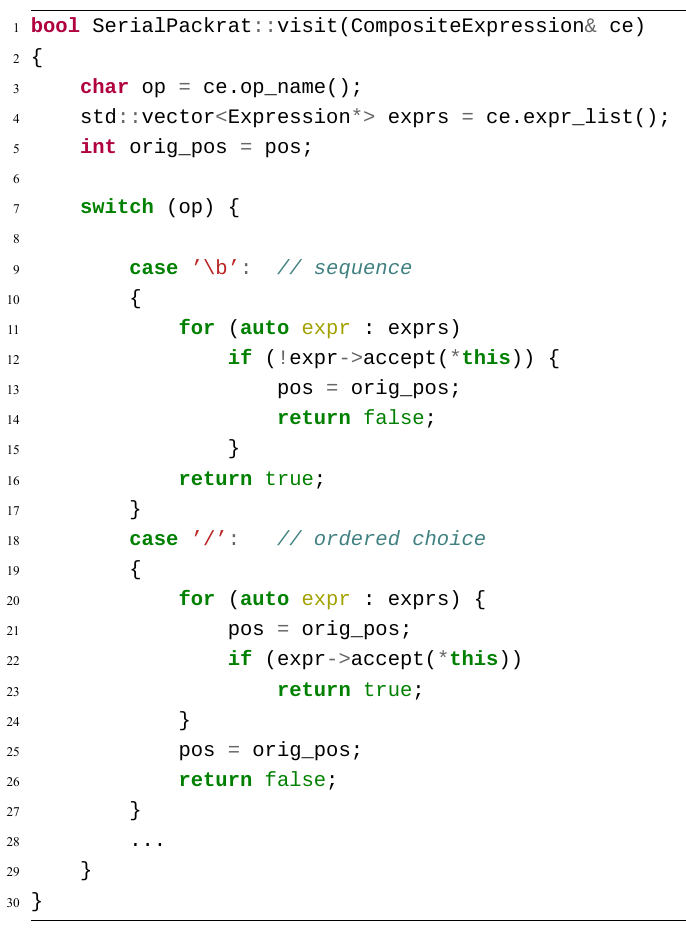
\includegraphics[width=0.50\textwidth]{pics/ce}
\end{figure} 
\end{frame}
\iffalse
\section{Γεννήτορας συντακτικών αναλυτών packrat}

\begin{frame}
  \frametitle{Κίνητρο}
  \begin{itemize}
	\item Για να πειραματιστούμε με τις υλοποιήσεις μας χρειαζόμαστε μία γραμματική από τον αληθινό κόσμο (π.χ. Java) \pause
	\item Θα ήταν πολύ δύσκολο να φτιάξουμε ένα instance της γραμματικής αυτής με το "χέρι"
	\item Θα έπρεπε να φτιάξουμε τα instances όλων των τερματικών, μη τερματικών, κανόνων κλπ. \pause
  \end{itemize}
  Λύση? \pause Parser Generator!
\end{frame}

\begin{frame}
  \frametitle{Pipeline}
    \centering
	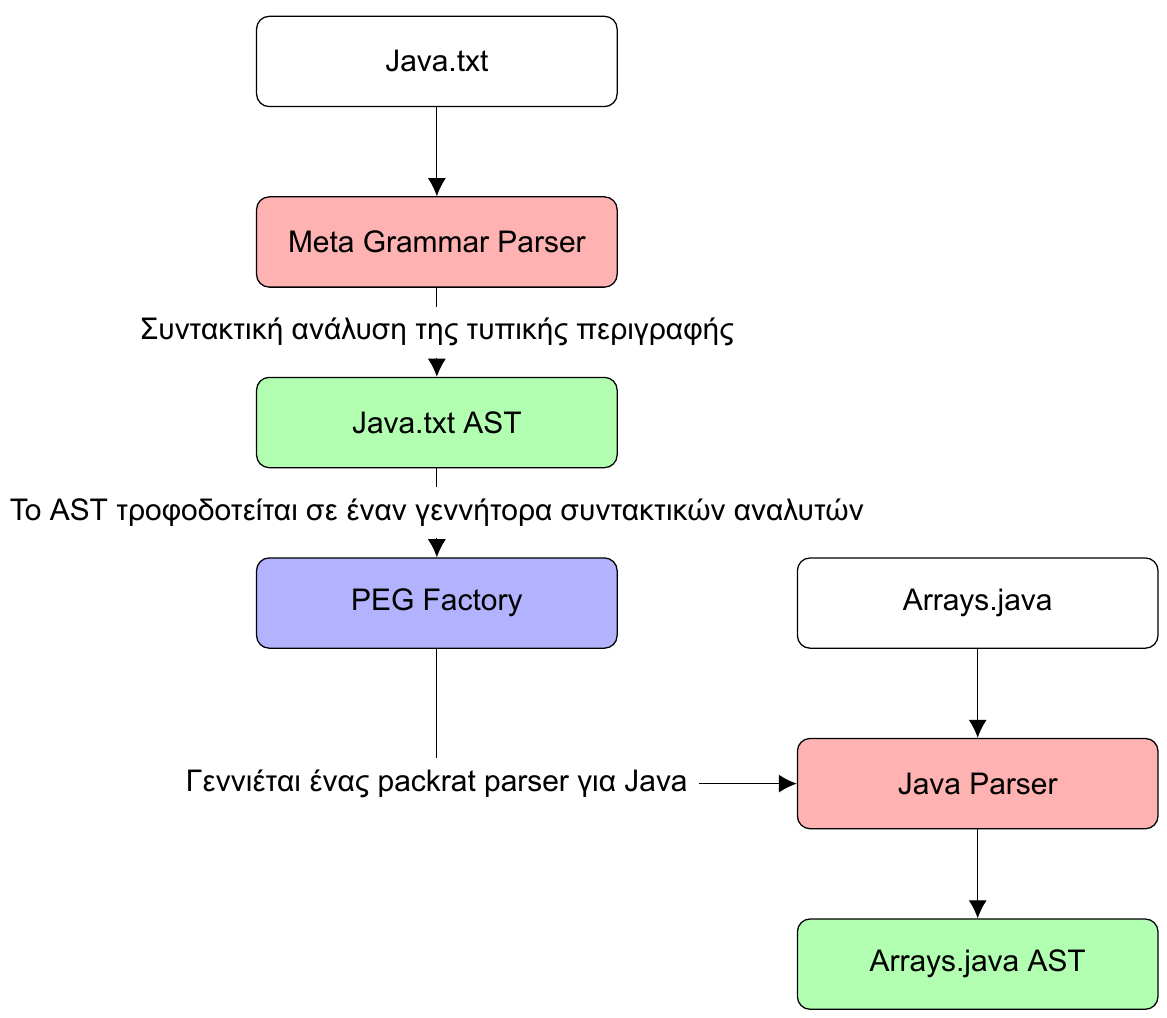
\includegraphics[width=0.75\textwidth]{pics/pipeline}
\end{frame}


\begin{frame}[fragile]
  \frametitle{Τυπική περιγραφή γραμματικής}
\begin{figure}[h]
    \centering
	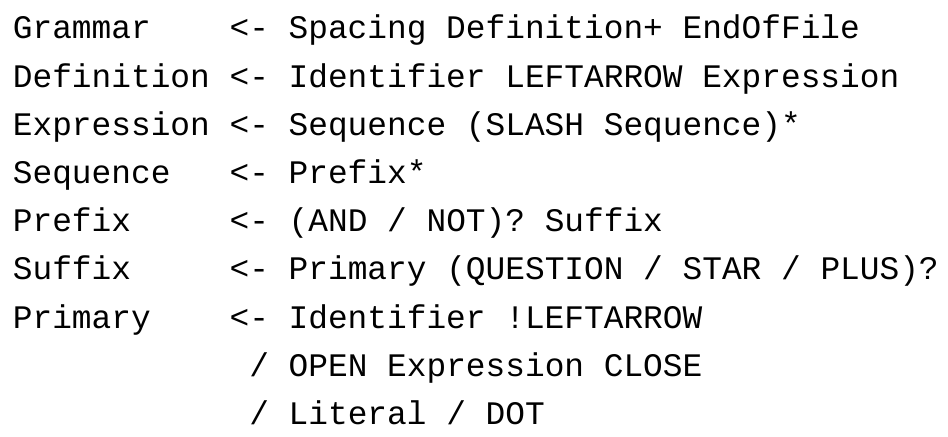
\includegraphics[width=0.80\textwidth]{pics/peg_spec}
\end{figure} 

\end{frame}

\begin{frame}
  \frametitle{Instance μίας μετα-γραμματικής}
\begin{figure}[h]
    \centering
	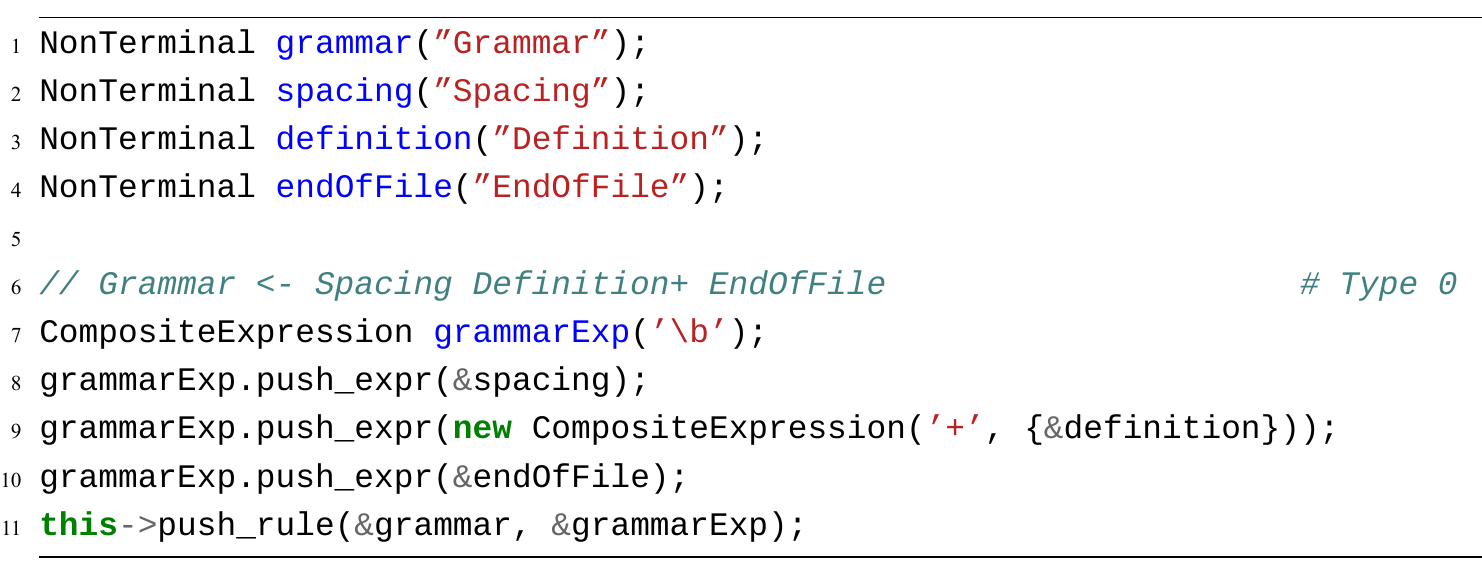
\includegraphics[width=0.95\textwidth]{pics/peg_instance}
\end{figure} 
\end{frame}

\begin{frame}
  \frametitle{Παράδειγμα: Java}
\begin{equation}
	Block \; \leftarrow \; LWING \; BlockStatements \; RWING
\end{equation}

\begin{figure}[h]
	\centering
\begin{tikzpicture}[%
  sibling distance=.5cm,
  empty/.style={draw=none},
  tlabel/.style={font=\footnotesize\color{red!70!black}}]
\Tree  [.Block
         [.LWING ]
         [.BlockStatements ]
         [.RWING ]
       ]

\end{tikzpicture}
\end{figure}
\end{frame}

\begin{frame}
  \frametitle{Διάσχιση - PEG Factory}
\begin{figure}[h]
    \centering
	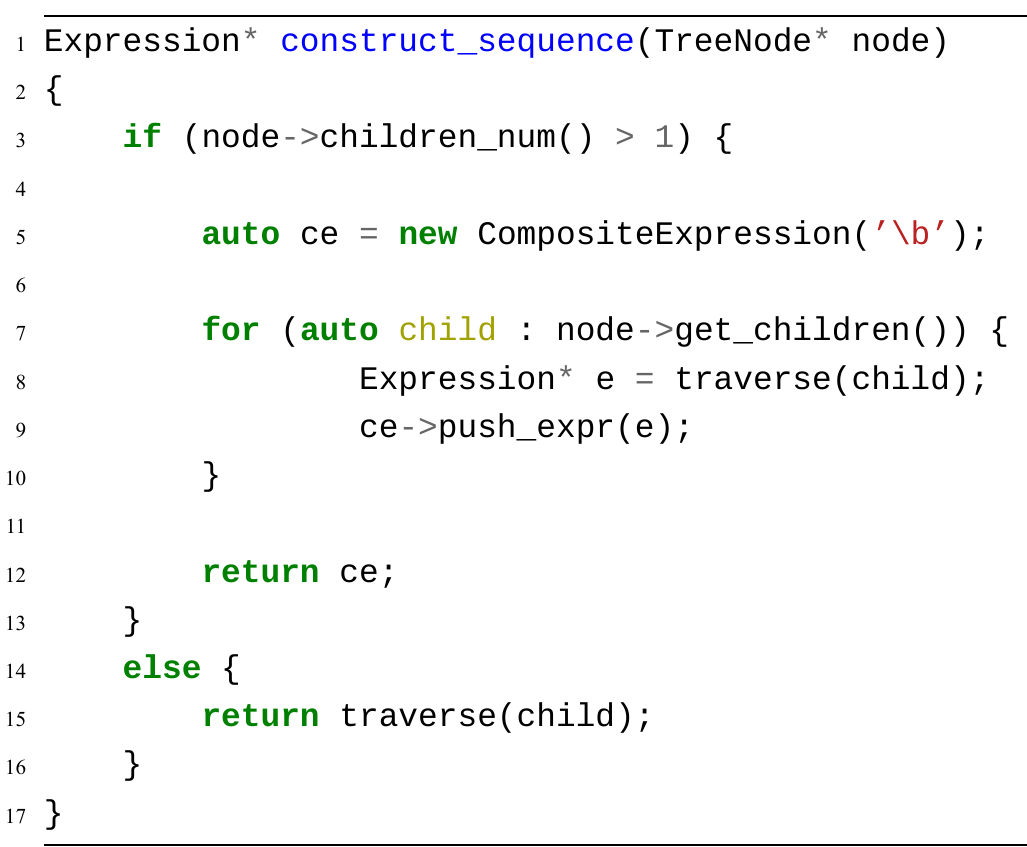
\includegraphics[width=0.60\textwidth]{pics/traverse}
\end{figure} 
\end{frame}

\begin{frame}
  \frametitle{Instance της γραμματικής-στόχου}
\begin{figure}[h]
    \centering
	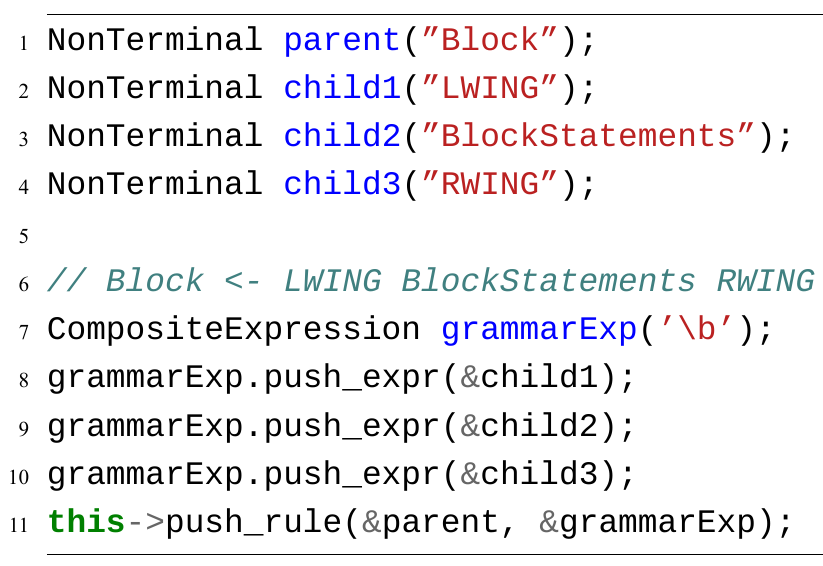
\includegraphics[width=0.60\textwidth]{pics/generated_instance}
\end{figure} 
\end{frame}
\fi
\section{Packrat Parsing με ελαστικό κυλιόμενο παράθυρο}

\begin{frame}
  \frametitle{Κίνητρο}
  \begin{itemize}
	\item O αλγόριθμος packrat καταναλώνει χώρο $O(NT * n)$, $NT$ ο αριθμός των μη τερματικών, $n$ το μήκος της εισόδου \pause
	\item Δεν ενδείκνυται για μεγάλα αρχεία εισόδου, καθώς ο πίνακας ενδιάμεσων αποτελεσμάτων μπορεί να γίνει απαγορευτικά μεγάλος \pause
	\item Χρειάζεται να τα κρατάμε όλα τα ενδιάμεσα αποτελέσματα? \pause
	\item Θα μπορούσαμε να μειώσουμε τις στήλες του πίνακα? \pause
	\item Τις γραμμές?
	\end{itemize}
  \end{frame}

\begin{frame}
  \frametitle{Μείωση των στηλών - Κυλιόμενο Παράθυρο}

	\begin{itemize}
	  \item Το πόσες στήλες πραγματικά χρειαζόμαστε εξαρτάται από το μήκος της μέγιστης οπισθαναχώρησης (έστω $w$)
	  \item Αν το γνωρίζαμε από πριν θα μπορούσαμε να έχουμε ένα παράθυρο που να "κυλάει" προς τα δεξιά ως προς την είσοδο \pause
	  \item $w = 1$: αλγόριθμος με backtracking, $w = n$: αλγόριθμος packrat \pause
	  \item Στην πράξη δεν ξέρουμε πόσο είναι, οπότε πρέπει να πειραματιστούμε \pause
	\end{itemize}

\begin{figure}[h]
    \centering
	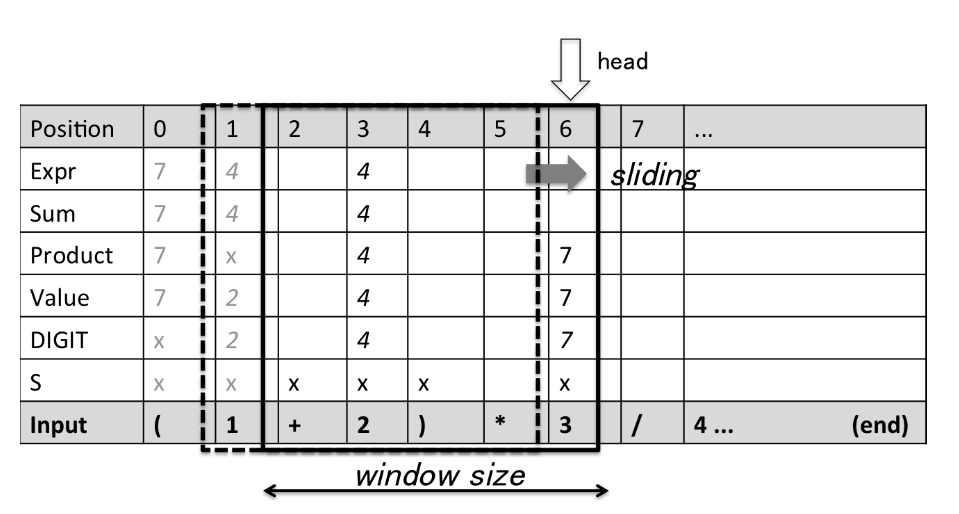
\includegraphics[width=0.60\textwidth]{../transcript/pics/slide_window}
\end{figure} 
\end{frame}

\begin{frame}
  \frametitle{Μείωση των γραμμών - Απενεργοποίηση μη τερματικών}

	\begin{itemize}
	  \item Το πόσες γραμμές πραγματικά χρειαζόμαστε εξαρτάται από το πόσο αξιοποιούνται τα αποτελέσματα των μη τερματικών
	  \item Θέτουμε ένα κατώφλι απενεργοποίησης $limit$
	  \item Αν μετά τις πρώτες $limit$ προσπελάσεις κελιών που αντιστοιχούν σε ένα μη τερματικό δεν αξιοποιήσουμε ούτε ένα αποτέλεσμα, σταματάμε να κρατάμε το μη τερματικό στον πίνακα
	\end{itemize}

\begin{figure}[h]
    \centering
	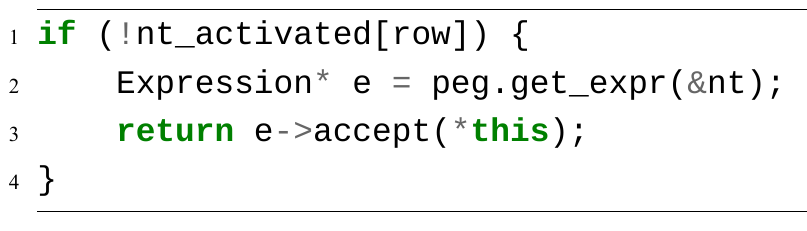
\includegraphics[width=0.60\textwidth]{pics/deactivated}
\end{figure} 
\end{frame}

\begin{frame}
  \frametitle{Συνδυασμός ιδεών: Elastic Packrat}
	\begin{itemize}
	  \item Χρησιμοποιούμε έναν μονοδιάστατο πίνακα $W*N$, όπου $W$ είναι το πλάτος του παραθύρου και $N$ ο αριθμός των ενεργών μη τερματικών.
	  \item Ακολούθως, χρησιμοποιούμε έναν δείκτη κατακερματισμού (hashing-based index) για να εντοπίσουμε σε ποιο σημείο του μονοδιάστατου πίνακα θα αποθηκευτεί το ενδιάμεσο αποτέλεσμα
	  \item<2-> Σταθερή μνήμη: $O(NT * W)$!
	\end{itemize}

\begin{figure}[h]
    \centering
	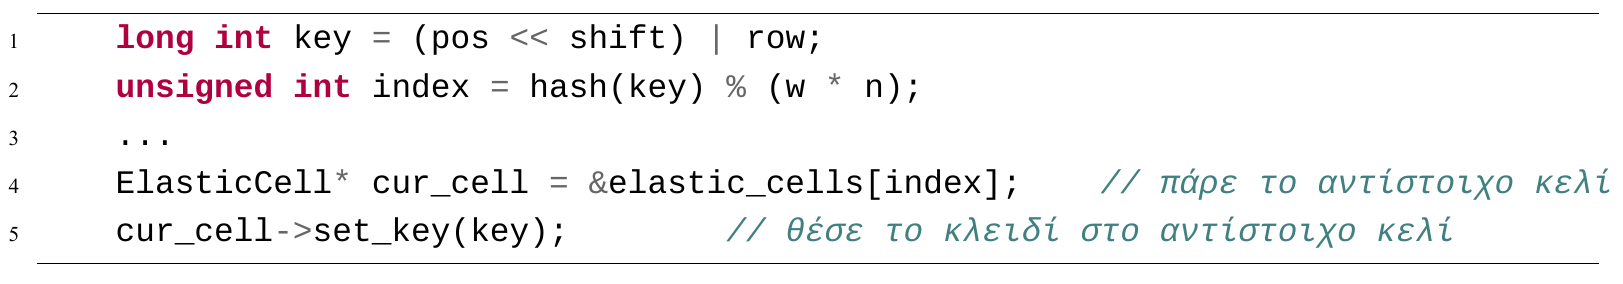
\includegraphics[width=1.10\textwidth]{pics/hash}
\end{figure} 

\end{frame}

\begin{frame}
  \frametitle{Elastic Packrat}
\begin{columns}

\column{0.6\textwidth}
Όταν απενεργοποιούμε ένα μη τερματικό ο χώρος του στον πίνακα μπορεί να αξιοποιηθεί από άλλα διευρύνοντας ουσιαστικά το παράθυρο

\column{0.5\textwidth}
\begin{figure}[h]
    \centering
	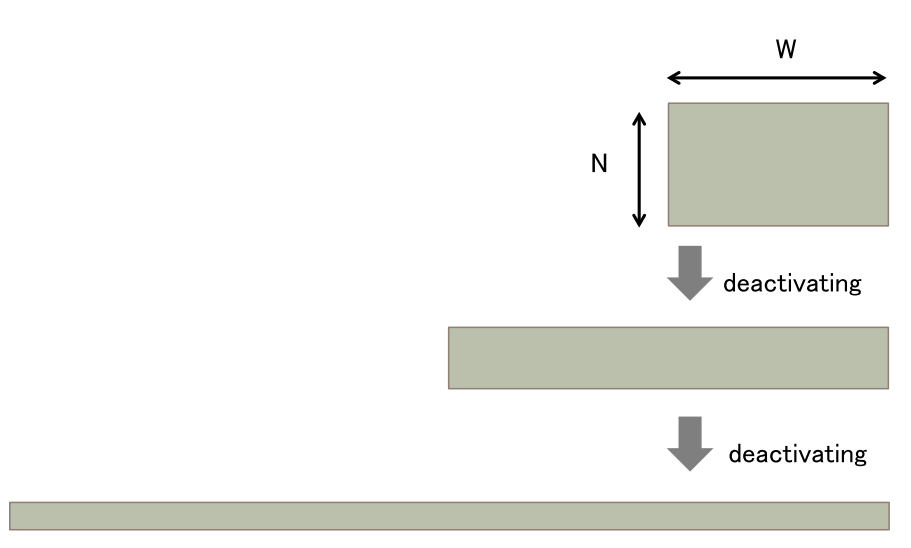
\includegraphics[width=1.00\textwidth]{../transcript/pics/elastic_slide_window}
\end{figure} 
\pause
\end{columns}

	\begin{itemize}
	  \item Μειονέκτημα του hashing-based index: πιθανές συγκρούσεις (collisions) μεταξύ διαφορετικών κλειδιών, που όμως αντιστοιχίζονται στο ίδιο index \pause 
	  \item Xάνεται η εγγύηση γραμμικού χρόνου \pause
	  \item Στην πράξη δουλεύει καλά και οδηγεί σε απλή υλοποίηση  \pause
	  \item Όσο προχωράμε στην είσοδο, τα νέα κελιά "εκτοπίζουν" τα παλιά που προσομοιώνοντας απλά την "κύλιση" του παραθύρου
	\end{itemize}
\end{frame}

\section{Παράλληλο Packrat Parsing}

\begin{frame}
  \frametitle{Ιδέα}
  \begin{itemize}
	\item Θέλουμε να βρούμε κάποιο κομμάτι του αλγορίθμου που μπορεί να εκτελεστεί από πολλά νήματα ταυτόχρονα, ώστε να μοιραστεί ο φόρτος εργασίας \pause
	\item Στη διατεταγμένη επιλογή $E \leftarrow E_1 / E_2 /  E_3$ οι υποεκφράσεις αναλύονται ξεκινώντας από το ίδιο σημείο της εισόδου  \pause
	\item Αν αποτύχει η $E_1$, τότε ξαναπροσπαθεί από το ίδιο σημείο η $E_2$ κλπ\pause
	\item Θεωρητικά θα μπορούσαμε να τις αναθέσουμε σε ξεχωριστά νήματα\pause
	\item Αναδρομική κλήση νημάτων: Αν κάποιο νήμα που κληθεί κατά την διατεταγμένη επιλογή πάει να αναλύσει με τη σειρά του διατεταγμένη επιλογή, καλεί και δικά του νήματα
  \end{itemize}

\end{frame}

\begin{frame}
  \frametitle{Λεπτά σημεία}
  \begin{itemize}
	\item Τα κελιά με τα ενδιάμεσα αποτελέσματα πρέπει να προστατεύονται από ταυτόχρονη χρήση\pause
	\item Αν το νήμα που ανέλυσε την $E_2$, επιστρέψει επιτυχώς, πρέπει πάλι να περιμένουμε το νήμα που αναλύει την $E_1$, καθώς η υποέκφραση αυτή έχει προτεραιότητα \pause
	\item Αν το νήμα που ανέλυσε την $E_i$, επιστρέψει επιτυχώς, πρέπει τερματίσουμε τα νήματα που ανέλαβαν τις $E_{i+1}, \dots, E_n$ \pause
	\item Aν υπάρχουν πολλές εναλλακτικές στην επιλογή, τότε ίσως να μην αξίζει να καλέσουμε πολλά νήματα, καθώς το overhead του fork-join θα είναι μεγάλο \pause
	\item Αν το βάθος του fork-join tree είναι ήδη μεγάλο, τότε ίσως πάλι να μην αξίζει να καλέσουμε νέα νήματα
  \end{itemize}
\end{frame}

\begin{frame}
  \frametitle{Λεπτά σημεία - Κλειδώματα}

  \begin{itemize}
	\item Για να αποφευχθούν συνθήκες ανταγωνισμού για τα κελιά πρέπει να προστατεύονται με κλειδώματα
	\item Ένας απλός και αποτελεσματικός τρόπος είναι κάθε κελί να έχει το κλειδί του οπότε για να το υπολογίσει κάποιος θα πρέπει να το κλειδώσει \pause

\begin{figure}[h]
    \centering
	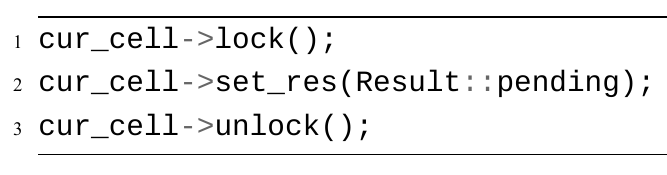
\includegraphics[width=0.60\textwidth]{pics/lock}
\end{figure} \pause
\item Όσο το κελί είναι pending (δηλαδή το υπολογίζει κάποιος) οι υπόλοιποι κάνουν busy-wait
  \end{itemize}
\end{frame}

\begin{frame}
  \frametitle{Λεπτά σημεία - Ιεραρχία}

  \begin{itemize}
	\item Κάθε νήμα που καλείται λαμβάνει έναν αριθμό $rank$ από το γονέα
	\item Υψηλότερο $rank$ είναι το $0$ \pause

\begin{figure}[h]
    \centering
	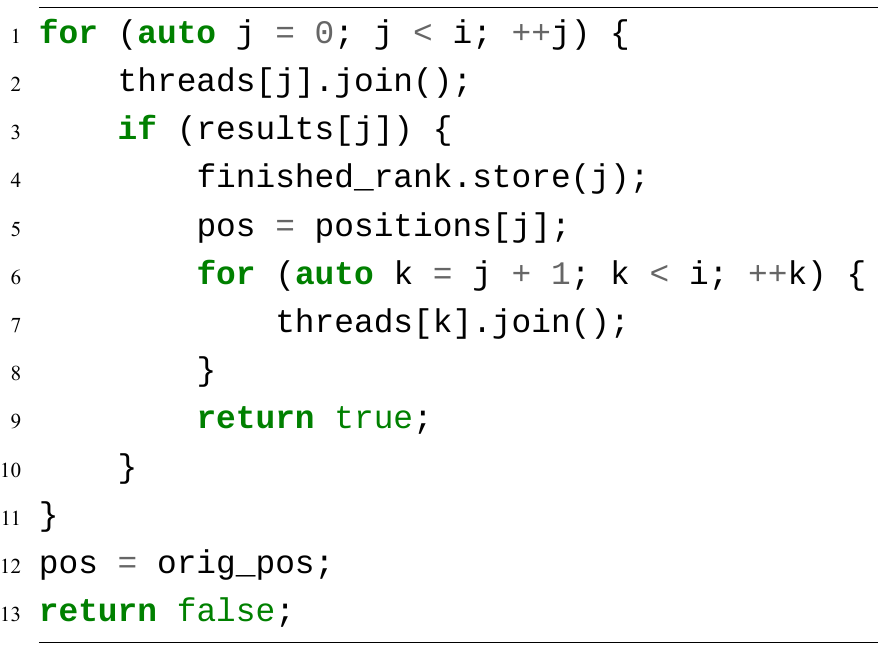
\includegraphics[width=0.75\textwidth]{pics/hierarchy}
\end{figure} 
  \end{itemize}
\end{frame}


\begin{frame}
  \frametitle{Λεπτά σημεία - Τερματισμός}

  \begin{itemize}
	\item Περιοδικός έλεγχος για πρόωρο τερματισμό από τον γονέα \pause
  \end{itemize}
\begin{figure}[h]
    \centering
	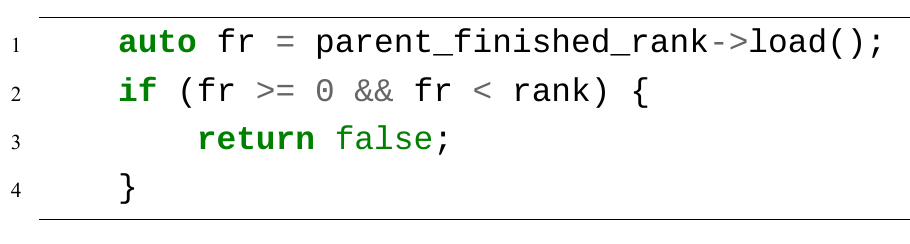
\includegraphics[width=0.60\textwidth]{pics/termination}
\end{figure} 
\end{frame}


\begin{frame}
  \frametitle{Όλα μαζί}

\begin{figure}[h]
    \centering
	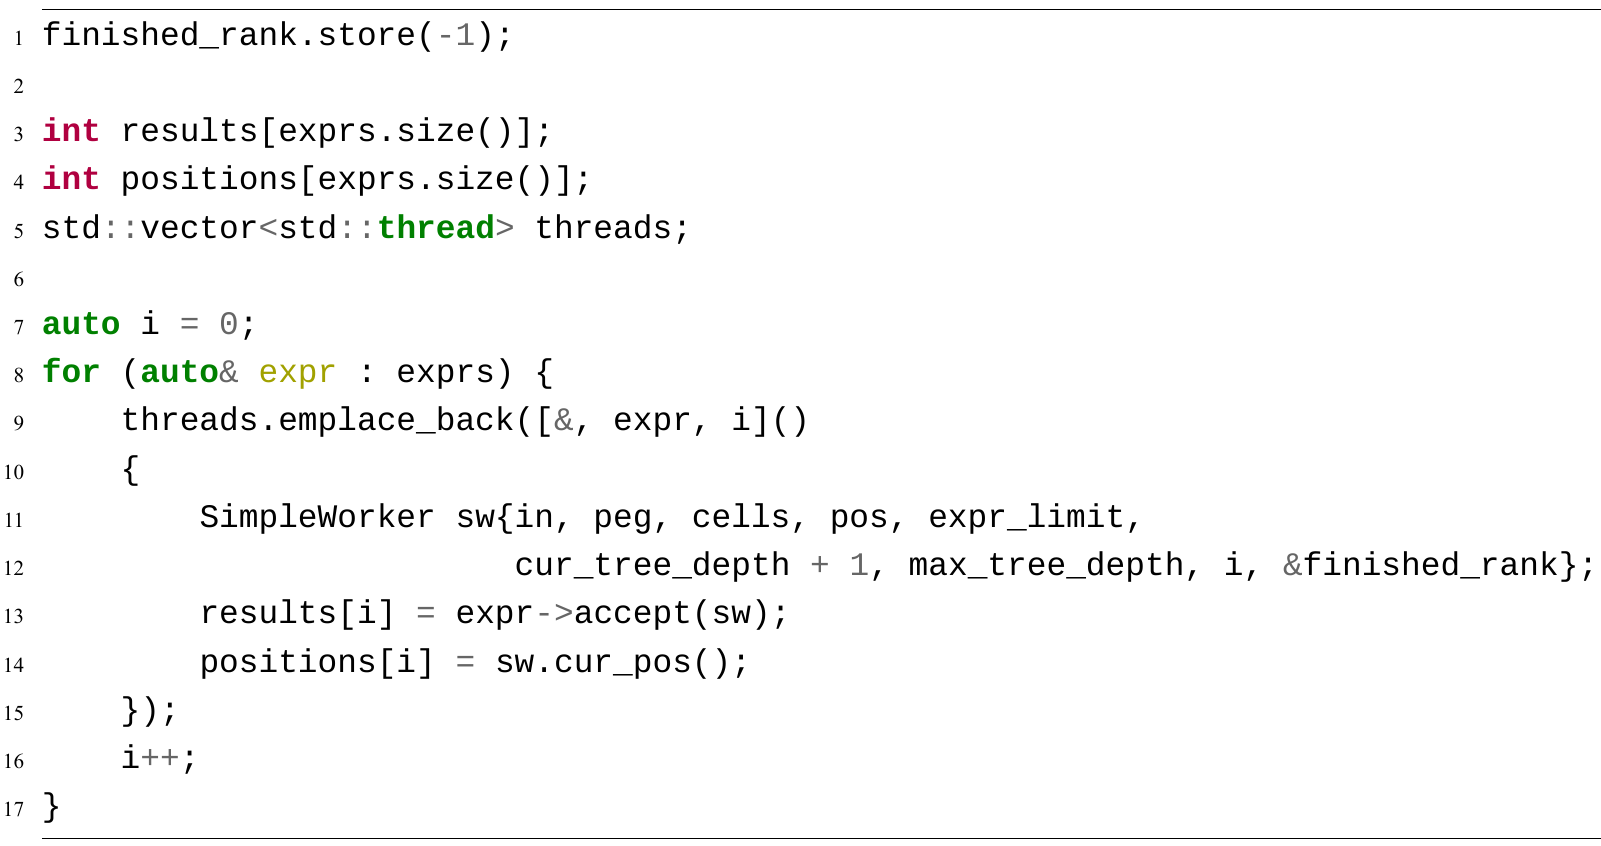
\includegraphics[width=1.05\textwidth]{pics/spawn}
\end{figure} 
\end{frame}

\section{Πειραματικά Αποτελέσματα}

\begin{frame}
  \frametitle{Δοκιμαστικά προγράμματα}
\begin{itemize}
  \item 3 αρχεία από τον πηγαίο κώδικα της Java
\begin{itemize}
  \item \textit{Arrays.java} - 116K 
  \item \textit{BigDecimal.java} - 140K 
  \item \textit{Throwable.java} - 28K 
\end{itemize}
\item Mέτριο προς μεγάλο μέγεθος ώστε να φανούν οι διαφορές στους χρόνους εκτέλεσης των αλγορίθμων
\item 12 νήματα διαθέσιμα
\item \textit{std::chrono::high\_resolution\_clock} της STL
\end{itemize}
\end{frame}

\begin{frame}
  \frametitle{Ρύθμιση των παραμέτρων}
  \begin{itemize}
	\item Τόσο για το elastic όσο και για το παράλληλο packrat εκτελούμε πειράματα για να βελτιώσουμε τους συνδυασμούς των παραμέτρων \pause
	\item Για το elastic δοκιμάζουμε παράθυρα μήκους $256$, $512, 1024$ και κατώφλια απενεργοποίησης $0, 16, 32, 48$ \pause
	  \begin{block}{Καλύτερος Συνδυασμός}
		$w = 256, thres = 32$
	  \end{block} \pause
	\item Για τον παράλληλο δοκιμάζουμε όρια μήκους διατεταγμένης επιλογής $2, 4, 6, 8$ και και μέγιστο βάθος δέντρου $1, 2$ \pause
	  \begin{block}{Καλύτερος Συνδυασμός}
		$expr\_limit = 4, max\_depth = 1$. Δηλαδή 5 ενεργά νήματα κατά το μέγιστο.
	  \end{block} 
  \end{itemize}
\end{frame}

\begin{frame}
  \frametitle{Τελική Σύγκριση}

\begin{table}[!ht]
\begin{tabular}{ |p{3cm}||p{2cm}|p{2cm}|p{2cm}|  }
 \hline
  \multicolumn{4}{|c|}{Χρόνοι εκτέλεσης (ms)} \\
 \hline
  Αλγόριθμος Packrat& Arrays ~~~  116K &BigDecimal 140K &Throwable 28K\\
 \hline
 Κλασικός & 404 & 350 & \cellcolor{green!45}46\\
  Elastic (256, 32) & \cellcolor{green!45}380 & \cellcolor{green!45}329 & 51\\
  Παράλληλος (1, 4) & 432 & 369 & 62\\
 \hline
\end{tabular}
  \caption{Τελικά αποτελέσματα για τους τρεις αλγορίθμους}
\end{table}

\end{frame}

\section{Συμπεράσματα}

\begin{frame}
  \frametitle{Συμπεράσματα}
  \begin{itemize}	
	\item Αδιαφιλονίκητος νικητής: elastic packrat \pause
	\item Καλύτερος χρόνος στα μεγάλα προγράμματα + σταθερή μνήμη \pause
	\item Στον παράλληλο δεν παρατηρείται επιτάχυνση (speedup) σε σχέση με τη σειριακή περίπτωση \pause
	\item H πράξη της διατεταγμένης επιλογής, παρόλο που θεωρητικά αφήνει χώρο για παράλληλη εκτέλεση, δεν συμπεριφέρεται τόσο καλά στην πράξη\pause
	\item Οverhead από fork-join\pause
	\item Ίσως πετυχαίνουν συχνά στη γραμματική μας οι πρώτες (αν όχι η πρώτη) επιλογή, οπότε μετά υπάρχει και ο επιπλέον χρόνος αναμονής νημάτων\pause
	\item Ο περιοδικός έλεγχος για τερματισμό αυξάνει το χρόνο εκτέλεσης
  \end{itemize}

\end{frame}

\begin{frame}
  \frametitle{Απορίες}
  \pause
\begin{center}
\huge Ευχαριστώ για την προσοχή σας!\footnotemark 
\end{center}
  \only<2->\footnotetext[1]{Hope you slept well!}
\end{frame}

\end{document}
